\documentclass{article}

\usepackage[italian]{babel}
\usepackage[utf8]{inputenc}
\usepackage[T1]{fontenc}
\usepackage{graphicx}
\usepackage{lipsum}
\usepackage{fancyhdr}
\usepackage{titlesec}
\usepackage{tocloft}
\usepackage{titling}
\usepackage{geometry}
\usepackage{float} % Per utilizzare l'opzione H nelle immagini
\usepackage{caption}
\usepackage{multicol} % molteplici colonne
\usepackage{todonotes}  % note
\usepackage{csvsimple} 

% Formattare codice
\usepackage{listings}
\lstset{language=Python}
\renewcommand{\lstlistingname}{Codice}

% Citazioni 
\usepackage{csquotes}
\usepackage[backend=biber, style=verbose]{biblatex}
\addbibresource{cit.bib}

% Riferimenti
\usepackage[noabbrev]{cleveref}
\crefname{figure}{Figura}{Figure}
\Crefname{figure}{Figura}{Figure}



% Configurazione label immagini
\DeclareCaptionLabelFormat{myformat}{#1~#2}
\captionsetup[figure]{labelformat=myformat}


% Box citazioni
\usepackage{tcolorbox}
\newtcolorbox[auto counter,number within=section]{mybox}[1][]{
    colback=white,
    colframe=black,
    sharp corners, 
    width=0.8\linewidth, 
    center title, 
    title={\textbf{Proprietà (\thetcbcounter)}},
    #1
}


% Margini
\geometry{a4paper, margin=2cm}

% Titolo
\title{Alberi Binari di Ricerca con Chiavi Duplicate}
\author{Niccolò Caselli}
\date{20/01/2024}
\renewcommand{\maketitlehooka}{\centering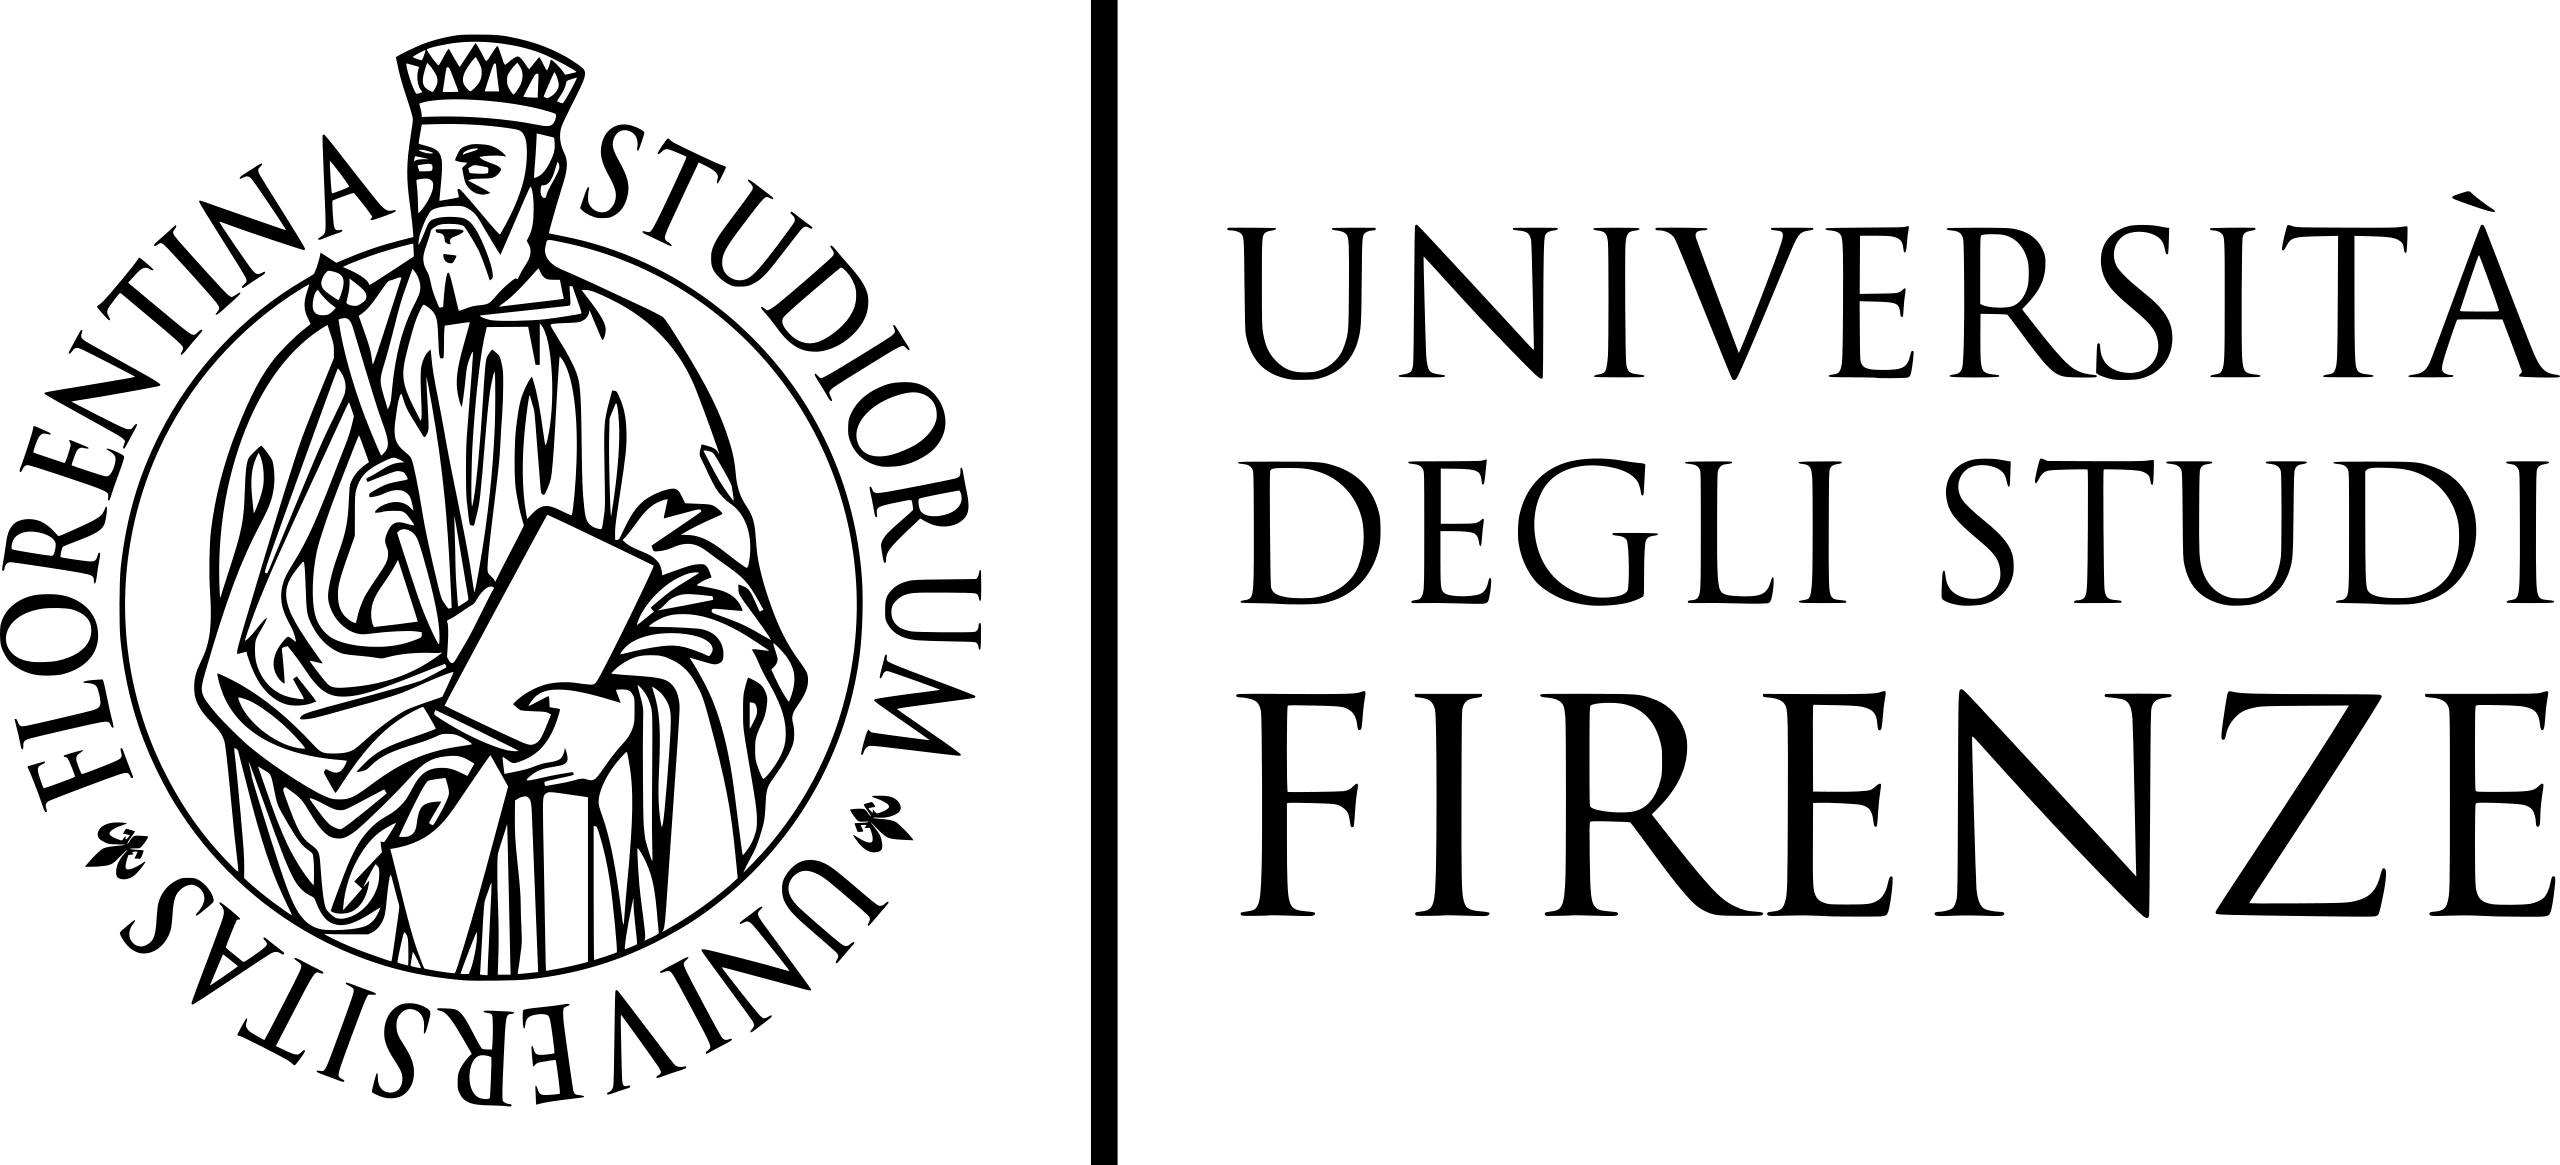
\includegraphics[width=0.5\textwidth]{logo}\vspace{1cm}}
\renewcommand{\maketitlehookb}{\centering\LARGE}
\renewcommand{\maketitlehookc}{\vspace{1cm}\centering\Large}

% Indice
\renewcommand{\cftsecleader}{\cftdotfill{\cftdotsep}}
\setlength{\cftbeforesecskip}{8pt}

% Configurazione degli stili di pagina
\pagestyle{fancy}
\fancyhf{}
\rhead{\thepage}
\lhead{\nouppercase{\leftmark}}
\renewcommand{\headrulewidth}{0.4pt}
\renewcommand{\footrulewidth}{0.4pt}

% Configurazione dei titoli delle sezioni
\titleformat{\section}[block]{\normalfont\Large\bfseries}{\thesection}{1em}{}
\titlespacing*{\section}{0pt}{\baselineskip}{\baselineskip}



\begin{document}

% PAGINA INIZIALE
\begin{titlepage}
  \maketitle
  \vspace*{\fill}
  \begin{center}
    \textbf{Relazione di Laboratorio di Algoritmi e Strutture Dati}
  \end{center}
  \vspace*{\fill}
\end{titlepage}


% INDICE
\renewcommand{\contentsname}{Indice} % Titolo dell'indice
\tableofcontents
\newpage

\section{Introduzione}
Nel contesto della struttura dati degli Alberi Binari di Ricerca, la presente relazione si propone di esaminare e confrontare diverse strategie implementative al fine di valutarne l'efficacia e l'impatto sulle prestazioni.
Gli Alberi Binari di Ricerca costituiscono una struttura fondamentale in molte applicazioni \textit{"real word"} ma, come vedremo in seguito, la gestione delle chiavi duplicate può essere complessa. Questa breve analisi si concentrerà su tre distinti approcci, non prima però di aver esposto brevemente il concetto di Albero Binario senza chiavi duplicate.
Saranno poi analizzati dei test di prestazioni sia dal punto di vista teorico, sia dal punto di vista empirico, per poi giungere alle conclusioni. 
La relazione è accompagnata da estratti di codice, tabelle riassuntive e grafici, e si invita inoltre a consultare i risultati allegati.
Infine, per chiarimenti sulle specifiche dei test si rimanda alla nota dell'ultimo paragrafo, seguito poi dalla bibliografia.

\section{Nozioni sugli Alberi Binari di Ricerca}

Prima di esaminare il problema delle chiavi duplicate cerchiamo di capire cos'è un albero binario di ricerca (abbreviato in BST dall'inglese \textit{Binary Search Tree}).

\begin{figure}[H]
  \centering
  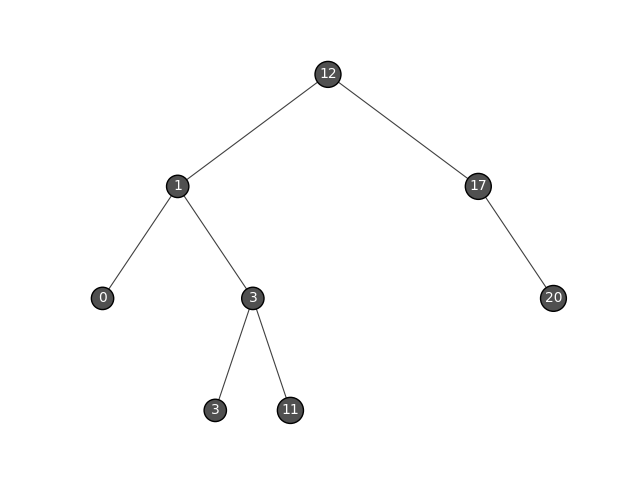
\includegraphics[width=0.7\textwidth]{./images/bst-generic}
  \caption{Esempio di albero binario di ricerca}
  \label{fig:bst-generic}
\end{figure}


\subsection{Cos'è un Albero Binario di Ricerca?}
\label{subsec:bst-introduction}
Un BST è un tipo di struttura dati basata su gli alberi, definiti nel libro  \emph{\citefield{cormen2023}{title}} come "grafi non orientati, connessi e aciclici".
Tale struttura ha la caratteristica di permettere l'esecuzione delle operazioni di base con complessità O(h), dove h è l'altezza dell'albero, proprietà che li rende efficienti per la realizzazione di dizionari, ricerca di valori, e attraversamenti. \\
Un albero binario di ricerca è costituito da una serie di nodi che nel calcolatore possono essere rappresentati con oggetti (e quindi classi) con i seguenti attributi:

\begin{itemize}
    \item una chiave (x.key)
    \item un puntatore al figlio sinistro (x.left)
    \item un puntatore al figlio destro (x.right)
    \item un puntatore al padre (x.p)
\end{itemize}

Enunciamo quindi la proprietà fondamentale di un albero binario di ricerca:

\begin{center}
\begin{mybox}
	\begin{itemize}
    \item Se y è nel sottoalbero sinistro di x, allora \(y.key < x.key\) 
     \item Se y è nel sottoalbero destro di x, allora \(y.key > x.key\) 
	\end{itemize}
\end{mybox}
\end{center}
\label{prop:bst-prop} 

Tale caratteristica dei BST è facilmente individuabile nell'albero di esempio di \cref{fig:bst-generic}. L'albero in figura ha però ha due nodi con stessa chiave, la chiave 3!
Come fare a gestire questa situazione? Sarà argomento del paragrafo \ref{sec:dup-section}.



\subsection{Implementazione in Python}

Come già accennato, in informatica possiamo rappresentare un albero binario con l'ausilio delle classi. Creiamo quindi una classe per rappresentare l'intero albero e una classe per il singolo nodo dell'albero. Tra queste due classi vi è quindi un relazione 
\textit{one-to-many}.

\vspace{5pt}

\begin{lstlisting}[language=Python, caption={Implementazione di un BST}, label=bst-implementation]


class Node:
    def __init__(self, key):
        self.key = key
        self.left = None
        self.right = None

class BST:
    def __init__(self):
        self.root = None

    # Imposta la radice dell'albero
    def setRoot(self, key):
        self.root = Node(key)

    # Inserisce un nodo nell'albero
    def insert(self, key):
        if (self.root is None):
            self.setRoot(key)
        else:
            self._insertNode(self.root, key)

    # Funzione di supporto per l'inserimento di un nodo
    def _insertNode(self, currentNode, key):
        if (key < currentNode.key):
            if (currentNode.left):
                self._insertNode(currentNode.left, key)
            else:
                currentNode.left = Node(key)
        elif (key > currentNode.key):
            if (currentNode.right):
                self._insertNode(currentNode.right, key)
            else:
                currentNode.right = Node(key)
\end{lstlisting}

\vspace{5pt}

Per ovvi motivi di impaginazione è stato riportato solo parte del codice; il lettore può quindi estenderlo a suo piacere implementando i metodi per gli attraversamenti dell'albero, la ricerca e tutto ciò che lo aggrada.
Come già sottolineato (Vedi \ref{subsec:bst-introduction}) il vantaggio di questa struttura dati è il costo asintotico delle sue operazioni di base. Più nello specifico, è evidente dalla funzione precedentemente mostrata che l'inserimento in un albero binario è un operazione che richiede $O(h)$ (dal momento che prima di inserire un nuovo nodo bisogna raggiungere una foglia percorrendo al più tutta l'altezza dell'albero - h). Lo stesso discorso si applica per la ricerca e la cancellazione (risulta invece diverso il caso degli attraversamenti - in ordine, posticipato e anticipato - che richiedono $\Theta(n)$).
Questo aspetto è fondamentale poiché spiega l'esigenza, su cui torneremo, di avere alberi il più possibili bilanciati. \\
È infine degna di nota la funzione che ho usato per la rappresentazione grafica dei BST in questa relazione.

\begin{lstlisting}[language=Python, caption={Rappresentazione Grafica di un BST}, label={lst:plot_tree}]
def plot_tree(tree):
    fig, ax = plt.subplots()
    _plot_tree(ax, tree.root, x=0, y=0, level=1)
    ax.axis('off')
    plt.show()

def _plot_tree(ax, node, x, y, level):
    if node is not None:
        ax.annotate(node.key, (x, y), xytext=(x, y),
                color="white",    
                ha='center',
                va='center', 
                bbox=dict(boxstyle='circle', fc='#505050')
        )

    xfactor = 1/2
    y_new = level * -2

    if node.left is not None:
        x_new = x - xfactor ** level
        ax.plot([x, x_new], [y, y_new], linewidth=.8,color="#404040")
        _plot_tree(ax, node.left, x_new, y_new, level + 1)

    if node.right is not None:
        x_new = x + xfactor ** level
        ax.plot([x, x_new], [y, y_new],  linewidth=.8, color="#404040")
        _plot_tree(ax, node.right, x_new, y_new, level + 1)
\end{lstlisting}


\section{Il Problema delle Chiavi Duplicate}
\label{sec:dup-section}
La definizione data fin'ora di Albero Binario di Ricerca si basa sulla fondamentale supposizione di unicità delle chiavi
(come implicito nella proprietà \ref{prop:bst-prop}).
Sappiamo però che questa ipotesi è difficilmente riscontrabile nelle applicazioni reali:
entriamo, dunque, nel merito del problema delle chiavi duplicate.

Possiamo trovare vari possibili approcci per gestire il problema, in questa discussione ne verranno trattati tre:  



\begin{itemize}
	\item Implementazione \textit{normale} (\ref{subsec:normal-implementation}).
	\item Implementazione con Flag Booleano (\ref{subsec:fag-implementation}).
	\item Implementazione con Lista Concatenata (\ref{subsec:list-implementation}).
\end{itemize}




\subsection{Premessa sulla ricerca}\label{subsec:search-int}Nonostante i test eseguiti e la relazione si concentreranno  sull'inserimento, è comunque necessario fare una premessa su cosa intendiamo come ricerca in un Albero Binario di Ricerca con chiavi duplicate. A seconda del tipo di utilizzo che vogliamo dare a un BST possiamo infatti realizzare in modi diversi la ricerca. In alcuni testi la ricerca di un nodo è descritta come un metodo che restituisce semplicemente se è presente o meno una specifica chiave in un albero o, in alternativa, che restituisce il primo nodo con tale chiave. In questi due specifici casi non bisogna mettere in pratica nessun accorgimento rispetto al caso senza chiavi duplicate; tuttavia, ciò è molto limitante: sebbene per motivi didattici quando si tratta i BST si tende a semplificare considerando ogni nodo solo caratterizzato dalla sua chiave, nella realtà, ogni nodo contiene anche dati satelliti. Ne consegue che sebbene due nodi possano avere una stessa chiave, il loro valore può essere diverso.
È il caso ad esempio dei dizionari; se in Javascript e Python non sono supportate le chiavi duplicate nei dizionari (oggetti in Javascript), un esempio valido sono invece le \textit{multimap} del c++ le quali, data una chiave, restituiscono tutti i valori associati a tale chiave. Questo è l'approccio seguito in questa relazione. 
 
\vspace{15px}
Ne approfitto quindi per includere qui la funzione di ricerca in BST senza chiavi duplicate, che verrà successivamente usata come riferimento.
 
\begin{lstlisting}[language=Python, caption={Ricerca in un BST senza chiavi duplicate},label={lst:bst-search}]
    def get(self, key):
        return self._getNode(self.root, key)

    def _getNode(self, currentNode, key):
        if (currentNode is None): return None
        if (key == currentNode.key): return currentNode
        if (key < currentNode.key):
            return self._getNode(currentNode.left, key)
        else:
            return self._getNode(currentNode.right, key)
\end{lstlisting} 
 
 
 
\subsection{Implementazione "normale"}\label{subsec:normal-implementation}
Un primo possibile approccio alla questione delle chiavi duplicate, e quello più immediato, è semplicemente aggiustare la definizione, volutamente ambigua, fornita precedentemente (vedi proprietà \ref{prop:bst-prop}).\\
Possiamo quindi riformulare la relazione tra i nodi di un BST affinché supporti l'inserimento quando la chiave da inserire è già presente nell'albero:

\begin{center}
\begin{mybox}
	\begin{itemize}
    \item Se y è nel sottoalbero sinistro di x, allora \(y.key \le x.key\) 
     \item Se y è nel sottoalbero destro di x, allora \(y.key > x.key\) 
	\end{itemize}
\end{mybox}
\end{center}
\label{prop:bst-normal-implementation-prop}

Questa modifica comporta quindi un cambiamento dell'implementazione dell'operazione di inserimento nella classe BST: al momento dell'inserimento i nodi con stessa chiave vengono inseriti nel sotto-albero di sinistra del primo nodo con tale chiave (e così via ricorsivamente). Aggiustiamo quindi il codice.

\begin{lstlisting}[language=Python, caption={Funzione ausiliaria di inserimento aggiornata}]
    def _insertNode(self, currentNode, key):
        if (key <= currentNode.key):
            if (currentNode.left):
                self._insertNode(currentNode.left, key)
            else:
                currentNode.left = Node(key)
        elif (key > currentNode.key):
            if (currentNode.right):
                self._insertNode(currentNode.right, key)
            else:
                currentNode.right = Node(key)
\end{lstlisting}



\begin{figure}[htbp]
  \begin{minipage}{0.5\textwidth}
    \centering
    \includegraphics[width=\linewidth]{./images/BST_UML}
    \caption{UML delle classi del BST}
    \label{fig:bst-normal-img1}
  \end{minipage}%
    \hspace{\columnsep}
      \hspace{\columnsep}
  \begin{minipage}{0.5\textwidth}
Ecco il diagramma delle classi per questa implementazione di Albero Binario. Come possibile vedere, ho deciso di implementare anche metodi di supporto e operazioni aggiuntive di cui non ho riportato il codice per motivi riassuntivi.
Stesso discorso per gli attributi, ho voluto aggiungere due variabili di supporto, \textit{find\_iterations\_count} e    \textit{insert\_iterations\_count}, per tenere traccia del numero i ricorsioni durante le operazioni, ovviamente solo al fine degli esperimenti.
  \end{minipage}
\end{figure}




In \cref{fig:bst-normal-img1} possiamo vedere l'albero derivante dall'inserimento ordinato dei seguenti elementi \(\mathbf{\{3, 1, 2, 2, 2, 4\}}\). Notiamo quindi che vi sono tre nodi con la stessa chiave 2, ognuno dei quali è nel sotto-albero sinistro del nodo padre con la medesima chiave.
\\
Non bisogna però cadere nella convinzione che nodi con stessa chiave si trovino sempre tutti adiacenti l'uno con l'altro.
A questo scopo si consideri la \cref{fig:bst-normal-img2}:  cambiando semplicemente l'ordine di inserimento dei valori della figura precedente (ora \(\mathbf{\{3, 2, 2, 1, 2, 4\}}\)) il risultato è molto diverso; tra il penultimo e l'ultimo nodo con chiave 2 vi è in mezzo un nodo con chiave 1!
Questo può portare a complicazioni nella ricerca.
Eviterò di mostrare anche il codice della ricerca, disponibile nel progetto allegato, ma questo dovrò essere un estensione del metodo già mostrato (Vedi codice \ref{lst:bst-search}); la differenza risiede nel fatto che, una volta trovata una chiave, bisogna rilanciare ricorsivamente sul ramo sinistro la medesima funzione. Infatti, come appena fatto notare dalla \cref{fig:bst-normal-img2} non siamo sicuri di aver trovato tutte le chiavi finché non arriviamo a una foglia. Creiamo quindi un array inizialmente vuoto e locale al metodo per poi passarlo come argomento alla funzione ausiliaria ricorsiva: una volta trovata una chiave duplicata verrà quindi messa nell'array. 
Il principale svantaggio di questa implementazione è che l'inserimento di tante chiavi uguali può tendere a sbilanciare l'albero il quale finisce per degenerare in una semplice lista. Infatti, è evidente che per creare l'albero di N elementi più sbilanciato possibile sia sufficiente inserire N volte la stessa chiave. Come in esempio (\cref{fig:bst-normal-img3}).


\begin{figure}[htbp]
  \begin{minipage}{0.5\textwidth}
    \centering
    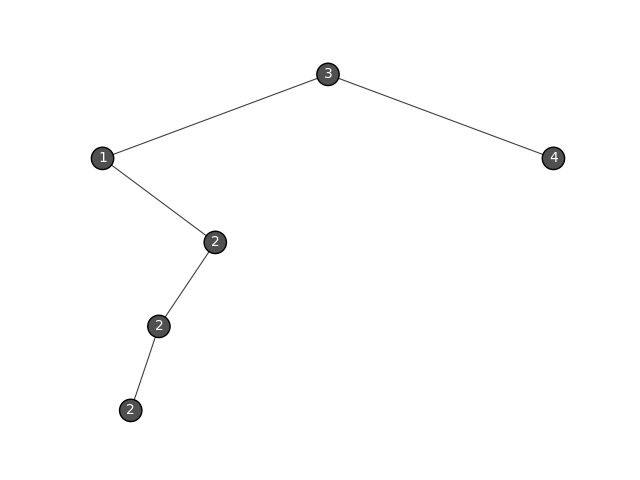
\includegraphics[width=\linewidth]{./images/bst-normal-img1}
    \caption{BST con chiavi duplicate}
    \label{fig:bst-normal-img1}
  \end{minipage}%
  \begin{minipage}{0.5\textwidth}
    \centering
    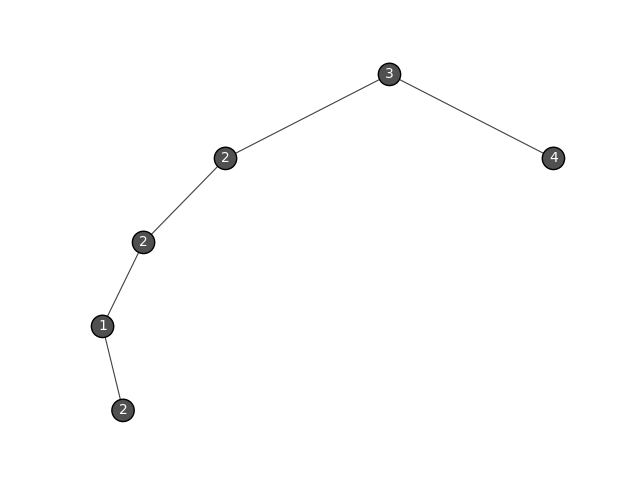
\includegraphics[width=\linewidth]{./images/bst-normal-img2}
    \caption{Altro esempio di BST con chiavi duplicate}
    \label{fig:bst-normal-img2}
  \end{minipage}
\end{figure}




\begin{figure}[H]
  \centering
  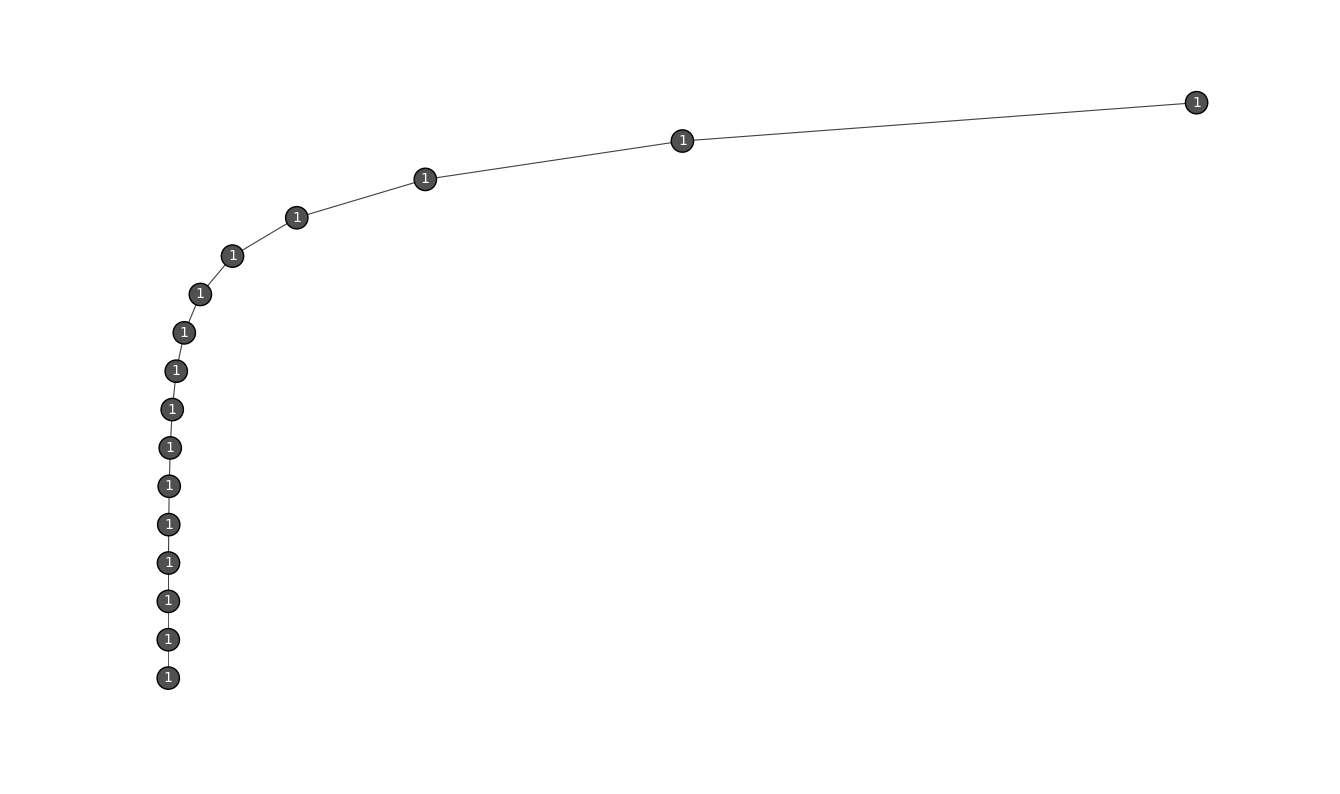
\includegraphics[width=0.7\textwidth]{./images/bst-normal-img3}
  \caption{Esempio di albero binario di ricerca sbilanciato}
  \label{fig:bst-normal-img3}
\end{figure}



\subsection{Metodo del Falg Booleano}
\label{subsec:fag-implementation}

Un altro possibile approccio al caso delle chiavi duplicate si basa su invece di inserire i nodi con chiave duplicate sempre a sinistra del nodo padre, farlo a sinistra o destra del padre a seconda di un flag booleano salvato nel nodo stesso. Più nello specifico: estendiamo la struttura dati di ogni nodo dell'albero così che il generico nodo x abbia un nuovo attributo \textit{x.flag} e quindi, durante l'inserimento di y, poniamo y a \textit{x.left} o \textit{x.right} a seconda del valore del flag, il quale viene alternato a ogni visita di x con chiave uguale. 

Il punto di forza di questa implementazione è il fatto che tende a preservare il bilanciamento dell'albero anche in presenza di molte chiavi duplicate, a differenza del primo approccio (Vedi \ref{subsec:normal-implementation}). Ciò risulta evidente se si prova a disegnare l'albero risultante dall'inserimento di N chiavi uguali (Vedi \cref{fig:bst-flag}).



\begin{figure}[H]
  \centering
  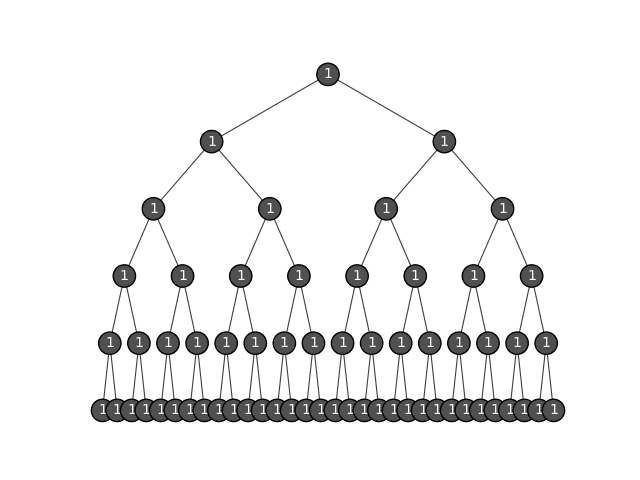
\includegraphics[width=0.7\textwidth]{./images/bst-flag}
  \caption{BST con Flag Booleano di 64 chiavi uguali}
  \label{fig:bst-flag}
\end{figure}



Per quanto riguarda il codice, le modifiche da apportare sono minime.
Aggiungiamo il nuovo attributo nella classe Nodo:

\begin{lstlisting}[language=Python, caption={Classe nodo di un BST con Flag Booleano}]
class Node:
    def __init__(self, key):
        self.key = key
        self.left = None
        self.right = None
        self.flag = False # <---
\end{lstlisting}

E aggiorniamo la funzione di supporto per l'inserimento:

\begin{lstlisting}[language=Python]
    def _insertNode(self, currentNode, key):        
        if(currentNode.key == key):
            if(currentNode.flag): self._insert_right(currentNode, key)
            else: self._insert_left(currentNode, key)
            currentNode.flag = not currentNode.flag # Alterna il flag
    
        if (key < currentNode.key): self._insert_left (currentNode, key)
        elif (key > currentNode.key): self._insert_right(currentNode, key)

    # Funzione di supporto per l'inserimento di un nodo a sinistra
    def _insert_left(self, currentNode, key):
        if (currentNode.left): self._insertNode(currentNode.left, key)
        else: currentNode.left = Node(key)

    # Funzione di supporto per l'inserimento di un nodo a destra
    def _insert_right(self, currentNode, key):
        if (currentNode.right): self._insertNode(currentNode.right, key)
        else: currentNode.right = Node(key)
\end{lstlisting}



La ricerca, invece si complica leggermente: come nel caso precedente se si trova un valore con chiave uguale si prosegue la ricerca, ma mentre nell'implementazione "normale" è sufficiente richiamare la ricorsione nel nodo a sinistra, in questo caso non abbiamo la certezza che i nodi con stessa chiave inseriti successivamente siano stati collocati a sinistra o a destra. Dobbiamo quindi proseguire la ricerca sia nel sotto-albero destro, sia nel sotto-albero sinistro.

\begin{figure}[htbp]
  \begin{minipage}{0.5\textwidth}
    \centering
    \includegraphics[width=\linewidth]{./images/BST_FLAG_UML}
    \caption{UML delle classi per BST con Flag Booleano}
    \label{fig:BST_FLAG_UML}
  \end{minipage}%
    \hspace{\columnsep}
      \hspace{\columnsep}
  \begin{minipage}{0.5\textwidth}
	Come evidente nel diagramma UML, ho deciso di implementare le modifiche sui nodi dell'albero estendendo la classe Nodo tramite ereditarietà. Avrei potuto fare la stessa cosa anche con la classe Albero, ma ho preferito evitare il polimorfismo di Python, non molto utilizzato.
  \end{minipage}
\end{figure}


\subsection{Metodo della Lista Concatenata}
\label{subsec:list-implementation}



L'ultimo approccio possibile trattato in questa relazione è quello  della lista concatenata: inseriamo tutti i nodi con chiave uguale in una lista concatenata.
Una possibile implementazione nel codice è di estendere la classe Nodo con un puntatore \textit{next} al prossimo elemento della lista concatenata. Nel mio caso ho aggiunto anche un campo   \textit{duplicates} che, nel primo nodo, tiene il conteggio dei nodi con chiave duplicata per esigenze rappresentative.

\begin{lstlisting}[language=Python, caption={Classe Nodo di un BST con lista concatenata}]
class Node:
    def __init__(self, key):
        self.key = key
        self.left = None
        self.right = None
        self.next = None # <---
        self.duplicates = 0 # <---
\end{lstlisting}

A questo punto, in fase di inserimento, se si trova un nodo con stessa chiave già esistente basta inserire il nuovo nodo.

\begin{lstlisting}[language=Python, caption={Gestione chiavi duplicate con lista concatenata}]
     if (key == currentNode.key):
            newNode = Node(key)
            newNode.next = currentNode.next
            currentNode.next = newNode
            currentNode.duplicates += 1

\end{lstlisting}

\vspace{15px}


\begin{figure}[H]
  \centering
  \includegraphics[width=0.5\textwidth]{./images/BST_LIST_UML}
    \caption{UML delle classi per BST con Lista Concatenata}
  \label{fig:BST_LIST_UML}
\end{figure}

\vspace{15px}

Apportando una semplice modifica alla funzione \textit{plot\_tree} (Vedi codice~\ref{lst:plot_tree}) possiamo visualizzare questo approccio in Figura \ref{fig:bst-list-img1} e Figura \ref{fig:bst-list-img2}.
Per ogni nodo è segnato tra parentesi il numero di occorrenze di quella chiave.

Per quanto concerne la ricerca, in questo approccio essa si semplifica notevolmente:
una volta trovato il primo nodo con la chiave voluta tramite il metodo esposto nel Codice \ref{lst:bst-search} sarà sufficiente scorrere la lista concatenata per avere tutti gli altri nodi con la medesima chiave.


\begin{figure}[htbp]
    \centering
  \begin{minipage}{0.48\textwidth}  % Riduci la larghezza della prima minipage
    \centering
    \includegraphics[width=\linewidth]{./images/bst-list-img1}
    \caption{BST con gestione chiavi duplicate tramite lista concatenata}
    \label{fig:bst-list-img1}
  \end{minipage}%
  \hfill  % Aggiungi uno spazio orizzontale tra le due colonne
  \begin{minipage}{0.48\textwidth}  % Riduci la larghezza della seconda minipage
    \centering
    \includegraphics[width=\linewidth]{./images/bst-list-img2}
    \caption{BST con lista concatenata di 100 chiavi uguali}
    \label{fig:bst-list-img2}
  \end{minipage}
\end{figure}




\section{Test delle prestazioni}
Entriamo ora nel dettaglio sulle prestazioni di queste tre possibili implementazioni.
Esaminiamo quindi il problema dell'inserimento di N chiavi identiche all'interno di un BST inizialmente vuoto e dell'operazione di ricerca, con N che tende a un numero molto grande.



\subsection{Analisi Teorica}

Come già discusso nel paragrafo \ref{subsec:normal-implementation} l'implementazione senza particolari accorgimenti ha il problema della degenerazione dell'albero in una lista nel caso di un elevato numero di inserimento con stessa chiave.
La teoria ci dice infatti che l'inserimento in un albero di ricerca è un operazione che richiede $O(h)$; tuttavia, come immaginabile dalla \cref{fig:bst-normal-img3}, nell'inserimento di n chiavi identiche si deve ogni volta arrivare in fondo all'albero di altezza $h=n$. Ne consegue che ci si aspetta un comportamento lineare $\Theta(n)$.
\\
Il secondo approccio del Flag Booleano (Paragrafo \ref{subsec:fag-implementation}) evita questa problematica e cerca di preservare il bilanciamento dell'albero. L'altezza diventa quindi funzione logaritmica e la complessità di l'inserimento $\Theta(log(n))$.
\\
Infine per quanto riguarda l'approccio tramite lista concatenata (Vedi \ref{subsec:list-implementation}) sappiamo che una volta trovato il primo nodo con chiave uguale, l'inserimento in testa alla lista concatenata è un'operazione $\Theta(1)$; dobbiamo però prima trovare tale nodo, il quale può anche non esistere. Abbiamo allora $O(h) + \Theta(1) = O(h)$. 
Tuttavia, nel caso del test di inserimento di n chiavi uguali l'albero degenera in un singolo nodo (Vedi Figura \ref{fig:bst-list-img2}) e quindi la complessità risultante diventa $\Theta(1) + \Theta(1) = \Theta(1)$.


\subsection{Risultati Sperimentali}

Come più volte ripetuto il test eseguito consiste nell'inserire N (numero molto grande) volte la stessa chiave in un albero binario di ricerca per comprendere in questo \underline{caso estremo} le differenze tra le tre implementazioni.
Ho strutturato il progetto in modo da evitare il più possibile la duplicazione di codice. Ho quindi creato una classe Albero per ognuno dei tre tipi e ho poi scritto una funzione di test che, preso in ingresso un'istanza di una qualsiasi classe albero, esegue i test di ricerca e inserimento su tale classe per un numero di volte passato come parametro, salvando poi i risultati sul disco in file \textit{xlsx} e \textit{csv}.\\
Il primo approccio, come ipotizzato nel paragrafo precedente, si è rilevato il più dispendioso di risorse computazionali e di tempo. Infatti, se i grafici generati per gli altri due casi arrivano all'inserimento in Alberi Binari di Ricerca di fino \underline{un milione} di elementi, nel caso dell'implementazione classica del BST il test è stato eseguito fino a un albero di \underline{200-mila elementi}. Come apprezzabile dal grafico riportato, il costo di questa operazione segue un andamento lineare e già i vari test sino a 200.000 chiavi hanno impiegato sul mio calcolatori (Vedi la nota sui test) più di mezz'ora di esecuzione. I test con N nell'ordine dei milioni, che ho più volte tentato, erano quasi non praticabili, e a mio avviso nemmeno significativi. Per i test è stata inoltre apportata una modifica alla classe Albero per tenere traccia del numero di iterazioni (in realtà se si vuole essere precisi, ricorsioni) che sono state necessarie per l'inserimento di ogni valore in un albero di dimensione n. Ad ogni dimensione dell'albero, quindi, sono stati salvati i tempi di esecuzione e il numero di iterazioni impiegate in un dizionario, ovvero un hash table di Python, utilizzando il valore corrente di n come chiave.
A conferma dell'andamento lineare dell'inserimento con il primo approccio è quindi anche il grafico del numero di iterazioni e, sopratutto, la tabella (\ref{tab:bst-insertion-summarised}) che ci mostra chiaramente l'identità tra il numero di elementi dell'albero e il numero di iterazioni necessarie per l'inserimento (questo ovviamente perché necessario scorrere tutto l'albero degenerato in una lista concatenata).


\begin{figure}[htbp]
 \begin{minipage}{0.5\textwidth}
    \centering
    \includegraphics[width=\linewidth]{./tests_output/bst/insertion.png}
    \caption{Prestazioni di inserimento di 200.000 chiavi identiche in un BST senza accorgimenti particolari}
    \label{fig:bst-normal-insetion}
  \end{minipage}
    \hspace{0.05\textwidth}
  \begin{minipage}{0.5\textwidth}
    \centering
    \includegraphics[width=\linewidth]{./tests_output/bst/insertion_iterations.png}
    \caption{Variazione del numero di iterazioni per l'inserimento in un BST di 200.000 chiavi identiche}
    \label{fig:bst-normal-insetion-iterations}
  \end{minipage}%
\end{figure}



\begin{minipage}[t]{\linewidth}
\begin{multicols}{2}
\begin{minipage}{\linewidth}
    \centering
    \csvautotabular{./tests_output/bst/insertion_summarised.cvs} % Percorso corretto per la prima tabella
    \captionof{table}{Risultati dell'inserimento in un BST normale}
    \label{tab:bst-insertion-summarised}
\end{minipage}
\columnbreak
\begin{minipage}{\linewidth}
    \centering
    \csvautotabular{./tests_output/bst/insertion_iterations_summarised.cvs} % Percorso corretto per la seconda tabella
    \captionof{table}{Numero di iterazioni nell'inserimento in un BST normale}
    \label{tab:bst-insertion-iterations-summarised}
\end{minipage}
\end{multicols}
\end{minipage}
\vspace{15px}



    \todo[inline, size=\small, backgroundcolor=gray!20, linecolor=gray, caption={\textit{}}]{\textbf{Nota sulle tabelle}. I test sono stati eseguiti su alberi di dimensioni fino a un milione di elementi e sono stati salvati i risultati in file \textit{.xlsx} da migliaia di righe. Ne consegue che, per ovvi motivi, questi file sono stati successivamente abbreviati da un altro script Python selezionando solo le misurazioni più significative. Si invita comunque a consultare i risultati allegati.}

\vspace{15px}

L'approccio del Flag Booleano da un punto di vista teorico dovrebbe dimostrarsi caratterizzato da una complessità logaritmica, tuttavia in questo caso diventa già molto più difficile interpretare il grafico.
Infatti, quando si parla di logaritmo spesso si tende a sottostimare quando questa funzione cresca lentamente: nel caso di 10.000 elementi sono necessarie solo 13 iterazioni per arrivare in fondo all'albero e inserire un nuovo valore; con un milione di elementi si sale ad appena a 19 iterazioni. Risulta evidente che per un calcolatore moderno la differenza, ad esempio, tra 13 o 19 iterazioni (e quindi di fatto confronti) è praticamente impercettibile e quindi il grafico risulta quasi costante e indistinguibile con quello del \textit{BST LIST}.
I test sono stati eseguiti su 1 milione di elementi e hanno impiegato un tempo quasi insignificante. Tuttavia, cercando di aumentare il numero di elementi ho riscontrato dei problemi con il terminale e l'editor di testo che sono andati in crash. Suppongo, mettendo le mani avanti poiché non ne posso avere la certezza, che questo sia un problema specifico dell'IDE, o della gestione del sistema o di Python delle chiamate ricorsive.

Nonostante ciò, dopo aver messo in atto piccoli accorgimenti alla visualizzazione del grafico e zoomando nella sezione di interesse, è possibile scorgere l'andamento logaritmico, anche se con molto rumore (dovuto probabilmente ad altri processi del calcolatore e in generale all'aleatorietà di tale tipo di test quando si va a considerare intervalli di tempo così ridotti).
Questo risulta ancora più evidente se si prende in considerazione il grafico delle iterazioni di inserimento.

\begin{figure}[htbp]
 \begin{minipage}{0.5\textwidth}
    \centering
    \includegraphics[width=\linewidth]{./tests_output/bst_flag/insertion.png}
    \caption{Prestazioni di inserimento di 1.000.000 chiavi identiche in un BST con Flag booleano}
    \label{fig:bst-flag-insetion}
  \end{minipage}
      \hspace{0.05\textwidth}
  \begin{minipage}{0.5\textwidth}
    \centering
    \includegraphics[width=\linewidth]{./tests_output/bst_flag/insertion_iterations.png}
    \caption{Ricorsioni nell'inserimento di 1.000.000 di chiavi identiche in un BST con Flag booleano}
    \label{fig:bst-flag-insetion-iterations}
  \end{minipage}%
\end{figure}

\vspace{10px}
L'approccio della Lista Concatenata deve avere come grafico un andamento costante, e così è. Nuovamente, risulta tuttavia di non immediata interpretazione: infatti, se rappresentiamo il grafico concentrandosi sulla zona di interesse, come nel caso di \cref{fig:bst-list-insetion}, poiché in questo caso l'operazione di inserimento risulta molto veloce e poco dispendiosa di risorse, accade che la variabile di incertezza/casualità influenza maggiormente il risultato.
Ecco perché il grafico in \cref{fig:bst-list-insetion} non risulta perfettamente come costante, ma i valori dei test si distribuiscono quasi uniformemente in un intervallo. È inoltre fondamentale notare come la scala verticale dei grafici di   \cref{fig:bst-list-insetion} e  \cref{fig:bst-flag-insetion} sia diversa; rispettivamente dell'ordine di 10e-6 per la prima e 10e-7 per la seconda, che quindi risulta più "zoomata". Analizzando le Tabelle \ref{tab:bst-flag-insertion-summarised} e \ref{tab:bst-list-insertion-summarised} emerge subito come l'ultimo approccio abbia prestazioni effettivamente quasi costanti e, sopratutto, di un ordine di grandezza 10 volte più piccolo dell'implementazione con Flag Booleano.


\begin{figure}[htbp]
 \begin{minipage}{0.5\textwidth}
    \centering
    \includegraphics[width=\linewidth]{./tests_output/bst_list/insertion.png}
    \caption{Prestazioni di inserimento di 1.000.000 di chiavi identiche in un BST con Lista Concatenata}
    \label{fig:bst-list-insetion}
  \end{minipage}
      \hspace{0.05\textwidth}
  \begin{minipage}{0.5\textwidth}
    \centering
    \includegraphics[width=\linewidth]{./tests_output/bst_list/insertion_iterations.png}
    \caption{Ricorsioni nell'inserimento di 1.000.000 di chiavi identiche in un BST con Lista concatenata}
    \label{fig:bst-list-insetion-iterations}
  \end{minipage}%
\end{figure}



\begin{minipage}[t]{\linewidth}
\begin{multicols}{2}
\begin{minipage}{\linewidth}
    \centering
    \csvautotabular{./tests_output/bst_flag/insertion_summarised.cvs} % Percorso corretto per la prima tabella
    \captionof{table}{Inserimento in un BST con Flag Booleano}
    \label{tab:bst-flag-insertion-summarised}
\end{minipage}

\columnbreak

\begin{minipage}{\linewidth}
    \centering
    \csvautotabular{./tests_output/bst_list/insertion_summarised.cvs} % Percorso corretto per la seconda tabella
    \captionof{table}{Inserimento in un BST con Lista Concatenata}
    \label{tab:bst-list-insertion-summarised}
\end{minipage}

\end{multicols}

\end{minipage}

\vspace{10px}

Vediamo infine ciò che è veramente significativo: la visualizzazione del confronto diretto tra i 3 approcci.
Risulta subito evidente come entrambi gli approcci della lista concatenata e del flag booleano, nonostante magari la necessità di una iniziale progettazione e implementazione più specifica, portano enormi benefici. Entrambi i grafici di  {\cref{fig:comparison_insertion}} e {\cref{fig:comparison_insertion_zommed}} sono stati realizzati sulla base degli stessi dati già mostrati; il secondo è però più zoomato sull'asse delle y  così che si possano apprezzare anche le misurazioni di \textit{BST FLAG} e \textit{BST LIST}, prticamente impercettibile nella figura {\cref{fig:comparison_insertion}} dominata dal grafico del primo approccio.

\begin{figure}[htbp]
 \begin{minipage}{0.5\textwidth}
    \centering
    \includegraphics[width=\linewidth]{./tests_output/comparison_insertion.png}
    \caption{Confronto tra le prestazioni di inserimento dei 3 tipi di BST}
    \label{fig:comparison_insertion}
  \end{minipage}
      \hspace{0.05\textwidth}
  \begin{minipage}{0.5\textwidth}
    \centering
    \includegraphics[width=\linewidth]{./tests_output/comparison_insertion_zommed.png}
    \caption{Zoom del confronto tra le prestazioni di inserimento dei 3 tipi di BST}
    \label{fig:comparison_insertion_zommed}
  \end{minipage}%
\end{figure}


\newpage

\begin{figure}[htbp]
  \begin{minipage}{0.32\textwidth}
    \centering
    \includegraphics[width=\linewidth]{./tests_output/bst/search.png}
    \caption{Prestazione di ricerca in un BST}
    \label{fig:search1}
  \end{minipage}
  \hfill
  \begin{minipage}{0.32\textwidth}
    \centering
    \includegraphics[width=\linewidth]{./tests_output/bst_flag/search.png}
    \caption{Prestazioni di ricerca in un BST con Flag Booleano}
    \label{fig:search2}
  \end{minipage}
  \hfill
  \begin{minipage}{0.32\textwidth}
    \centering
    \includegraphics[width=\linewidth]{./tests_output/bst_list/search.png}
    \caption{Prestazioni di ricerca in un BST con Lista Concatenata}
    \label{fig:search3}
  \end{minipage}
\end{figure}

Durante lo svolgimento di questi test, per ognuno dei tre tipi di BST e per gli stessi valori di n, è stata anche eseguita l'operazione di ricerca (Vedi premessa nel paragrafo \ref{subsec:search-int}).
Tuttavia, come ci si poteva aspettare \underline{in questo specifico caso} i risultati ottenuti non sono per nulla significativi.
Ho deciso di limitare i test a soli 1000 elementi, un campione di dati significativamente ridotto ma comunque sufficiente per lo scopo. È di banale evidenza, infatti, che nel modo in cui si è intesa la ricerca, devono essere trovate tutte le occorrenze  della chiave, ma essendo il test su alberi composti solo da tale chiave dovrà essere attraversato ogni nodo. Il costo della ricerca cresce quindi linearmente con l'aumentare di n, come si può evincere dai grafici riportati (\cref{fig:search1}, \cref{fig:search2}, \cref{fig:search3}).

 

\subsection{Cenni sulla cancellazione}
Per quanto riguarda l'operazione di cancellazione, se non è stata inclusa nei test è perché ritengo che non sia significativa nell'ottica di questo studio.
Brevemente: è noto come la cancellazione in un BST si articola su vari possibili casi; se il nodo da cancellare non ha figli o solo un figlio sarà sufficiente eliminare il nodo e trasferire il figlio al nodo padre. Le cose si complicano se il nodo da eliminare ha sia figlio destro, sia figlio sinistro: non entrerò nel dettaglio, ma è necessario eseguire una o due operazioni di trapianto a seconda se il successore del nodo è l'immediato figlio destro o no. Ciò che conta è che l'operazione ha un costo di \textit{O(h)} senza però contare la ricerca del nodo da cancellare. Quello che cambia tra i tre alberi è quindi la ricerca, già trattata, e il fatto che se nei primi due approcci dopo aver eliminato il primo nodo bisogna continuare la ricerca per eliminare anche gli altri, il terzo approccio ha il vantaggio che per cancellare tutti i nodi  con la stessa chiave è sufficiente eliminare solo il primo di nodo.

\section{Conclusioni}
È giunto il momento delle conclusioni. Tengo a sottolineare nuovamente come i test eseguiti rappresentino il caso peggiore e quindi un caso  di utilizzo ben oltre l'estremo che in situazione reali difficilmente si presenta. Sarebbe stato opportuno generare quindi un dataset meno sbilanciato in termini di chiavi duplicate, ma non avrebbe reso con tale chiarezza le differenze tra i tre alberi. Il test ha reso chiaro come se il primo approccio è immediato e semplice nella sua implementazione, questo non è per nulla efficiente nella gestione delle chiavi duplicate se in grande numero. Il secondo approccio migliora notevolmente il bilanciamento dell'albero nel caso di molte chiavi duplicate e quindi di conseguenza le prestazioni, non più lineari ma logaritmiche. La sua pecca però consiste in un'implementazione che complica ulteriormente la ricerca.
Infine, l'ultimo approccio è quello che sicuramente ha avuto prestazioni migliori durate i test, persino lineari!  Non è però così tutto semplice, poiché questo risultato è legato esclusivamente alla natura del test eseguito. Ciò comunque non esclude che tale approccio, a fronte di un'implementazione più onerosa in termini di accorgimenti necessari, possa offrire effettivamente ottime prestazioni anche i casi di uso reali, stando anche qui ovviamente attenti a non far degenerare l'albero in una semplice lista.
Per finire quindi, la scelta delle implementazioni ovviamente non è immediata, ma va decisa sulla base di vari fattori tra cui il tipo di operazioni che interessa eseguire sulla struttura dati e sopratutto la quantità di elementi con chiave duplicata che si stima di avere. 


\newpage

% PC 
\section*{Nota sui test}
\addcontentsline{toc}{section}{Nota sui test}

Si tenga presente che per svolgere i test discussi è necessario alzare il limite massimo di ricorsione di default di Python. Questo è necessario per prevenire che l'interprete blocchi l'esecuzione di un elevato numero di chiamate ricorsive, però necessarie in questa tipologia di test.
Per fare ciò basta impostare un nuovo limite nel seguente modo:
\begin{lstlisting}[language=Python]
sys.setrecursionlimit(500000000)
\end{lstlisting}


\vspace{20pt}


Si tenga inoltre presente che tutti i test presenti in questa relazione sono stati eseguiti su un calcolatore con le seguenti specifiche:

\begin{multicols}{2}
    \textbf{Hardware:}
    \begin{itemize}
        \item \textbf{Modello:} MacBook Pro 2022
        \item \textbf{CPU:} Apple Silicon M2 (8 core)
        \item \textbf{RAM:} 8 GB LPDDR5 (Micron)
    \end{itemize}
    
    \columnbreak
    
    \textbf{Software:}
    \begin{itemize}
        \item \textbf{Versione macOS:} 14.0
        \item \textbf{Versione Python:} 3.11.4
        \item \textbf{Versione Pip3:} 23.3.2
    \end{itemize}
\end{multicols}

\vspace{20pt}

% BIBLIOGRAFIA 
\printbibliography[heading=bibintoc, title={Bibliografia}]  



\end{document}
